\section{Introduction}
Let us first briefly describe finite difference methods and finite element methods used to solve the 
following boundary value problem
\begin{equation}
\label{laplace}
-\Delta u = f,  \mbox{ in } \Omega,\quad
u=0  \mbox{ on } \partial\Omega,\quad
\Omega=(0,1)^2.
\end{equation}
For the $x$ direction and the $y$ direction, we consider the partition:
\begin{equation}\label{partitionyx}
 0=x_0<x_1<\cdots<x_{n+1}=1, \quad x_j=\frac{j}{n+1},\quad (j=0,\cdots,n+1);
 \end{equation}
 \begin{equation}\label{partitiony}
 0=y_0<y_1<\cdots<y_{n+1}=1, \quad y_j=\frac{j}{n+1},\quad (j=0,\cdots,n+1).
\end{equation}
Such a uniform partition in the $x$ and $y$ directions leads us to a special example in two dimensions, 
a uniform square mesh $\R_h^2 = \big\{(mh,nh); n, m \in \Z\big\}$ (Figure \ref{fig:2dpartition}). 
Let $\Omega_h = \Omega\cap\R_h^2$, the set of interior mesh points and $\partial\Omega_h = \partial\Omega\cap\R_h^2$, the set of boundary mesh points.

\begin{figure}
\begin{center}
\setlength{\unitlength}{0.5mm}
\begin{picture}(45,45)(50,0)
\linethickness{0.25mm}
\multiput(0,0)(10,0){6}{\line(0,1){50}}
\multiput(0,0)(0,10){6}{\line(1,0){50}}
\put(0,0){\line(1,1){50}}
\put(10,0){\line(1,1){40}}
\put(20,0){\line(1,1){30}}
\put(30,0){\line(1,1){20}}
\put(40,0){\line(1,1){10}}
\put(0,10){\line(1,1){40}}
\put(0,20){\line(1,1){30}}
\put(0,30){\line(1,1){20}}
\put(0,40){\line(1,1){10}}
\put(47,34){$\displaystyle \left. \begin{array}{l}~ \\ ~\end{array}
\right\} h={1\over n+1}$}
\put(54,14){$\displaystyle N = n^2$}
\multiput(100,0)(10,0){6}{\line(0,1){50}}
\multiput(100,0)(0,10){6}{\line(1,0){50}}
\put(147,34){$\displaystyle \left. \begin{array}{l}~ \\ ~\end{array}
\right\} h={1\over n+1}$}
\put(154,14){$\displaystyle N = n^2$}
\end{picture}
\setlength{\unitlength}{0.5mm}
\end{center}
\label{fig:2dpartition}
\caption{Two-dimensional uniform grid for finite element and finite difference}
\end{figure}

\subsection{Five-point finite difference methods}
We can use the center difference to approximate the derivatives as follows:
$$
\frac{\partial^2 u}{\partial x^2}(x_i,y_j)=
\frac{u(x_{i+1},y_j)-2u(x_i,y_j)+u(x_{i-1},y_j)}{h^2}+{\mathcal O}(h^2),
$$
$$
\frac{\partial^2 u}{\partial y^2}(x_i,x_j)=
\frac{u(x_{i},y_{j+1})-2u(x_i,y_j)+u(x_{i},y_{j-1})}{h^2}+{\mathcal
 O}(h^2). 
$$
Thus, 
\begin{equation}\label{2dfd-truncation}
(-\Delta_hu)(x_i,y_j)=(-\Delta u)(x_i,y_j)+{\mathcal O}(h^2)
\end{equation}
where $-\Delta_h$ is a discretized operator for $-\Delta$ given by 
\begin{equation}
  \label{Delta-h}
(-\Delta_hu)(x_i,y_j)= \frac{1}{h^2}(4u(x_i,y_j)-(u(x_{i+1},y_j)+u(x_{i-1},y_j)
+u(x_i,y_{j+1})+u(x_i,y_{j-1}))).
\end{equation}
The truncation error \eqref{2dfd-truncation} can be proved by applying Taylor's expansion directly.

The finite difference scheme is then formed by
\begin{equation}
  \label{2d-fd0}
4u_{ij}-(u_{i+1,j}+u_{i-1,j}+u_{i,j+1}+u_{i,j-1})=f_{i,j},~~u_{i,j}=0~~\hbox{if}~~i ~~\hbox{or}~~ j\in \{0, n+1\}
\end{equation}
where 
\begin{equation}
  \label{fij-fd}
f_{i,j} =h^2 f(x_i, y_j).
\end{equation}

\begin{proposition}
The mapping $A$ in \eqref{uniform-laplace} has following properties
\begin{enumerate}
\item $A$ is symmetric, namely 
$$
(Au, v)_F=(u,Av)_F, ~~~\hbox{where}~~~ (u,v)_F=\sum_{i,j=1}^nu_{i,j}v_{i,j}.
$$
\item  $(Av, v)_F>0, ~~~\hbox{if}~~~v\neq 0.$
\item  $\rho(A)\le 8$.
\end{enumerate}
\end{proposition}

\subsection{Finite element methods}
We consider two finite elements: continuous linear element and bilinear element. These two finite element methods find $u_h\in V_h$ such that
$$
(\nabla u_h, \nabla v_h)=(f, v_h),\ \forall v_h\in V_h.
$$
The basis functions $\phi_{i,j}\in V_h$ such that 
\begin{equation*}
\phi_{i,j}(x_k,y_l)=\delta_{(i,j), (k,l)}=
\left\{
\begin{array}{rl}
1& (i,j)= (k,l)\\
0& (i,j)\neq (k,l)
\end{array}
\right.
\end{equation*}
The above formulation can be written as 
$$
Au=f,
$$
with $A_{(j-1)n+i, (l-1)n+k}=(\nabla \phi_{kl}, \nabla \phi_{ij})$ and $f_{(j-1)n+i, (l-1)n+k}=(f, \phi_{ij})$.
\begin{enumerate}
\item Continuous linear finite element discretization of
\eqref{laplace} on the left triangulation in Fig \ref{fig:2dpartition}. The discrete space for linear finite element is 
$$
V_h=\{v_h: v_h|_K\in P_1(K) \text{ and } v_h \text{ is continuous on each interior edge}\}.
$$ 
The basis functions according to the three vertice on the element below are $1-x$, $y$ and $x-y$.
%Here we need to notice that, $n_\ell = 2^{k_\ell} + 1$ for general PDEs grid 
%with the above boundary condition. For general images, we can take them as
%discrete functions on grid with size $n_\ell = 2^{k_\ell}m$ with small $m = 1,3,\cdots$.
%Then generally speaking, the coarse grid size is $n_{\ell+1} = \frac{n_\ell}{2}=2^{k\ell - 1}m$.
It is easy to verify that the formulation for the linear element method is exactly the same as the five-point finite difference scheme, namely 
\begin{equation}
  \label{2d-fe0}
4u_{ij}-(u_{i+1,j}+u_{i-1,j}+u_{i,j+1}+u_{i,j-1})=f_{i,j},~~u_{i,j}=0~~\hbox{if}~~i ~~\hbox{or}~~ j\in \{0, n+1\}.
\end{equation}
The linear finite element method solves
\begin{equation}
\label{laplace}
Au=f
\end{equation}
with
\begin{equation}
  \label{2d-fd}
A=tridiag (-I, B, -I), \quad B=tridiag (-1, 4, -1).
\end{equation}
The matrix $A$ is a block tridiagonal matrix. 

\begin{figure}[!ht]
\begin{center}
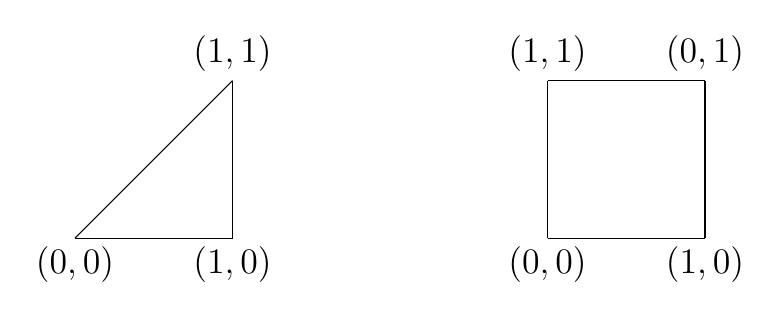
\begin{tikzpicture}[xscale=2,yscale=2]
\tikzstyle{every node}=[font=\Large,scale=0.9]
\draw[-] (0,0) -- (1,0);
\draw[-] (0,0) -- (1,1);
\draw[-] (1,0) -- (1,1);
\node[below] at (0,0) {$(0,0)$};
\node[below] at (1,0) {$(1,0)$};
\node[above] at (1,1) {$(1,1)$};
\draw[-] (3,0) -- (4,0);
\draw[-] (3,0) -- (3,1);
\draw[-] (4,0) -- (4,1);
\draw[-] (3,1) -- (4,1);
\node[below] at (3,0) {$(0,0)$};
\node[below] at (4,0) {$(1,0)$};
\node[above] at (3,1) {$(1,1)$};
\node[above] at (4,1) {$(0,1)$};
\end{tikzpicture}
\end{center}
\end{figure}
\item Continuous bilinear finite element discretization of
\eqref{laplace} on the right mesh in 
Fig. \ref{fig:2dpartition}. The discrete space for linear finite element is 
$$
V_h=\{v_h: v_h|_K\in \{1,\ x,\ y,\ xy \} \text{ and } v_h \text{ is continuous on each interior edge}\}.
$$ 
The basis functions according to the four vertice on the element above 
are $\frac{1}{4}(1-x)(1-y)$, $\frac{1}{4}(1+x)(1-y)$, $\frac{1}{4}(1-x)(1+y)$ and $\frac{1}{4}(1+x)(1+y)$. 
And we have
\begin{equation}
  \label{2d-fe1}
8u_{ij}-(u_{i+1,j}+u_{i-1,j}+u_{i,j+1}+u_{i,j-1}+u_{i+1,j+1}+u_{i-1,j-1}+u_{i-1,j+1}+u_{i+1,j-1})=f_{i,j},
\end{equation}
and 
$$
u_{i,j}=0~~\hbox{if}~~i ~~\hbox{or}~~ j\in \{0, n+1\}.
$$

The bilinear finite element method solves
\begin{equation}
\label{laplace-h}
Au=f
\end{equation}
with
%Here we need to notice that, $n_\ell = 2^{k_\ell} + 1$ for general PDEs grid 
%with the above boundary condition. For general images, we can take them as
%discrete functions on grid with size $n_\ell = 2^{k_\ell}m$ with small $m = 1,3,\cdots$.
%Then generally speaking, the coarse grid size is $n_{\ell+1} = \frac{n_\ell}{2}=2^{k\ell - 1}m$.
\begin{equation}\label{uniformbilinear-laplace}
\tilde A=
\begin{pmatrix}
\tilde A_1&\tilde A_2&\\
\tilde A_2&\tilde A_1&\tilde A_2&\\
     &\ddots&\ddots&\ddots&\\
     &     &\tilde A_2&\tilde A_1&\tilde A_2\\
     &     &     &\tilde A_2&\tilde A_1
\end{pmatrix},
\end{equation}
\begin{equation*}
\tilde A_1=
\begin{pmatrix}
8&-1&\\
-1&8&-1&\\
     &\ddots&\ddots&\ddots&\\
     &     &-1&8&-1\\
     &     &     &-1&8
\end{pmatrix},
\tilde A_2=
\begin{pmatrix}
-1&-1&\\
-1&-1&-1&\\
     &\ddots&\ddots&\ddots&\\
     &     &-1&-1&-1\\
     &     &     &-1&-1
\end{pmatrix},
\end{equation*}
\end{enumerate}


